\documentclass{article}
\usepackage[margin=1in]{geometry}
\usepackage{amsmath,amsthm,amssymb}
\usepackage{bbm,enumerate,mathtools}
\usepackage{tikz,pgfplots}
\usepackage{chessboard}
\usepackage[hidelinks]{hyperref}
\usepackage{multicol} % Problem 35

\newenvironment{question}{\begin{trivlist}\item[\textbf{Question.}]}{\end{trivlist}}
\newenvironment{note}{\begin{trivlist}\item[\textbf{Note.}]}{\end{trivlist}}
\newenvironment{references}{\begin{trivlist}\item[\textbf{References.}]}{\end{trivlist}}
\newenvironment{related}{\begin{trivlist}\item[\textbf{Related.}]\end{trivlist}\begin{enumerate}}{\end{enumerate}}


\begin{document}
  Consider all $r$-colorings of the $n \times m$ grid where no two colors
  are adjancent (horizontally/vertically) more than once.

\begin{figure}[!h]
  \centering
  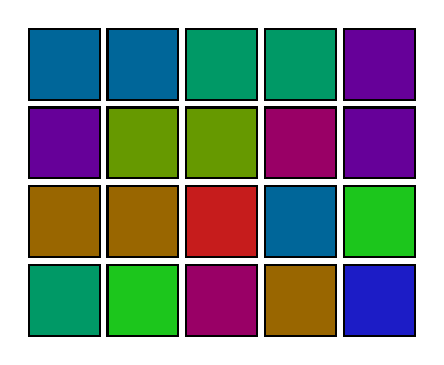
\begin{tikzpicture}
    \def\polyomino{
      0/3/0/2/3, 1/3/0/2/3, 2/3/0/3/2, 3/3/0/3/2, 4/3/2/0/3,
      0/2/2/0/3, 1/2/2/3/0, 2/2/2/3/0, 3/2/3/0/2, 4/2/2/0/3,
      0/1/3/2/0, 1/1/3/2/0, 2/1/7/1/1, 3/1/0/2/3, 4/1/1/7/1,
      0/0/0/3/2, 1/0/1/7/1, 2/0/3/0/2, 3/0/3/2/0, 4/0/1/1/7
    }

    \foreach \x/\y/\r/\g/\b in \polyomino {
      \draw[thick,fill={rgb:red,\r;green,\g;blue,\b}] (\x - 0.45, \y - 0.45) rectangle (\x + 0.45, \y + 0.45);
    }
  \end{tikzpicture}\\
  \caption{A $9$-coloring of the $4 \times 5$ grid where no two colors are adjancent
    more than once. There is no $8$-coloring.}
\end{figure}

\begin{question}
  Let $a(n, m)$ be the minimal $r$ such that there exists an $r$-coloring of the
  $n \times m$ grid. What is $a(n, m)$?
\end{question}
\begin{related}
  \item What if colors are not allowed to be self-adjacent?
  \item How many $a(n, m)$-colorings exist up to permutation of the colors?
  \item What if this is done on a triangular or hexagonal grid?
  \item What if orientation matters?
    (A horizontal adjacency is distinct from a vertical adjacency.)
  \item What if order matters? (red-green is distinct from green-red.)
  \item What if diagonal adjacencies are considered?
\end{related}

\begin{references}
  \item Problem 27.
  \item Problem 40.
  \item Problem 56.
\end{references}
\end{document}
